\documentclass[usenames,dvipsnames,tikz]{standalone}
\usepackage{amsmath,amssymb}
\usepackage{xcolor}
\colorlet{tBlue}{RoyalBlue!35!Cerulean}
\colorlet{tRed}{Red}
\usepackage{tikz}
\usepackage{standalone}
\begin{document}
	
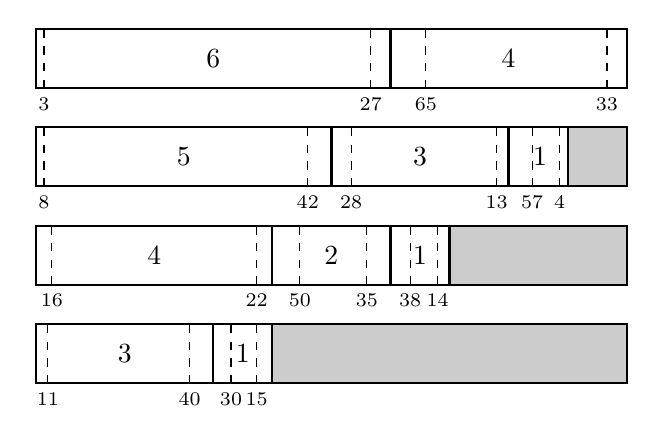
\begin{tikzpicture}
%\draw [help lines] (-1,-2) grid (12,5);
% 1=0.1, 2=0.15, 3=0.2, 4=0.25, 5=0.3
% 6 (3-27), 5 (8-42), 4 (33-65), 4 (16-22), 3 (13-28), 3 (11-40), 2 (35-50), 1 (15-30), 1 (14-38), 1 (4-57).

\draw [thick] (0,0) rectangle (7.5,0.75);
\draw [thick] (0,1.25) rectangle (7.5,2);
\draw [thick] (0,2.5) rectangle (7.5,3.25);
\draw [thick] (0,3.75) rectangle (7.5,4.5);

% Bottom row, 3, 1 (11-40, 30-15, sixth, tenth)
\draw [thick] (2.25,0) -- (2.25,0.75);
\draw [thick] (3,0) -- (3,0.75);
\filldraw[fill=black!20!white, draw=black, thick] (3,0) rectangle (7.5,0.75);
\draw [dashed] (0.15,0) -- (0.15,0.75);
\draw [dashed] (1.95,0) -- (1.95,0.75);
\draw [dashed] (2.475,0) -- (2.475,0.75);
\draw [dashed] (2.8,0) -- (2.8,0.75);
\node [below] at (0.15,0) {\scriptsize{11}};
\node [below] at (1.95,0) {\scriptsize{40}};
\node [below] at (2.475,0) {\scriptsize{30}};
\node [below] at (2.8,0) {\scriptsize{15}};
\node at (1.125,0.375) {3};
\node at (2.625,0.375) {1};

% Second from bottom row, 4, 2, 1 (16-22, 50-35, 38-14, fourth, seventh, ninth)
\draw [thick] (3,1.25) -- (3,2);
\draw [thick] (4.5,1.25) -- (4.5,2);
\draw [thick] (5.25,1.25) -- (5.25,2);
\filldraw[fill=black!20!white, draw=black, thick] (5.25,1.25) rectangle (7.5,2);
\draw [dashed] (0.2,1.25) -- (0.2,2);
\draw [dashed] (2.8,1.25) -- (2.8,2);
\draw [dashed] (3.35,1.25) -- (3.35,2);
\draw [dashed] (4.2,1.25) -- (4.2,2);
\draw [dashed] (4.75,1.25) -- (4.75,2);
\draw [dashed] (5.1,1.25) -- (5.1,2);
\node [below] at (0.2,1.25) {\scriptsize{16}};
\node [below] at (2.8,1.25) {\scriptsize{22}};
\node [below] at (3.35,1.25) {\scriptsize{50}};
\node [below] at (4.2,1.25) {\scriptsize{35}};
\node [below] at (4.75,1.25) {\scriptsize{38}};
\node [below] at (5.1,1.25) {\scriptsize{14}};
\node at (1.5,1.625) {4};
\node at (3.75,1.625) {2};
\node at (4.875,1.625) {1};

% Second from top row, 5, 3, 1 (8-42, 28-13, 57-4, second, fifth, eighth)
\draw [thick] (3.75,2.5) -- (3.75,3.25);
\draw [thick] (6,2.5) -- (6,3.25);
\draw [thick] (6.75,2.5) -- (6.75, 3.25);
\filldraw[fill=black!20!white, draw=black, thick] (6.75,2.5) rectangle (7.5,3.25);
\draw [dashed] (0.1,2.5) -- (0.1,3.25);
\draw [dashed] (3.45,2.5) -- (3.45,3.25);
\draw [dashed] (4,2.5) -- (4,3.25);
\draw [dashed] (5.85,2.5) -- (5.85,3.25);
\draw [dashed] (6.3,2.5) -- (6.3,3.25);
\draw [dashed] (6.65,2.5) -- (6.65,3.25);
\node [below] at (0.1,2.5) {\scriptsize{8}};
\node [below] at (3.45,2.5) {\scriptsize{42}};
\node [below] at (4,2.5) {\scriptsize{28}};
\node [below] at (5.85,2.5) {\scriptsize{13}};
\node [below] at (6.3,2.5) {\scriptsize{57}};
\node [below] at (6.65,2.5) {\scriptsize{4}};
\node at (1.875,2.875) {5};
\node at (4.875,2.875) {3};
\node at (6.4,2.875) {1};

% Top row, 6,4 (3-27, 65-33, first, third)
\draw [thick] (4.5,3.75) -- (4.5,4.5);
\draw [dashed] (0.1,3.75) -- (0.1,4.5);
\draw [dashed] (4.25,3.75) -- (4.25,4.5);
\draw [dashed] (4.95,3.75) -- (4.95,4.5);
\draw [dashed] (7.25,3.75) -- (7.25,4.5);
\node [below] at (0.1,3.75) {\scriptsize{3}};
\node [below] at (4.25,3.75) {\scriptsize{27}};
\node [below] at (4.95,3.75) {\scriptsize{65}};
\node [below] at (7.25,3.75) {\scriptsize{33}};
\node at (2.25,4.125) {6};
\node at (6,4.125) {4};

\end{tikzpicture}

\end{document}